% Template for ICASSP-2010 paper; to be used with:
%          mlspconf.sty  - ICASSP/ICIP LaTeX style file adapted for MLSP, and
%          IEEEbib.bst - IEEE bibliography style file.
% --------------------------------------------------------------------------
\documentclass{article}
\usepackage{amsmath,graphicx,02460, hyperref,float}
\usepackage[font=small,skip=1pt]{caption} %for the weird space betwween the caption and figures
\setlength\belowcaptionskip{-2ex} %for the weird space between the text and figures

\toappear{02456 Deep Learning, DTU Compute, Fall 2017}


\graphicspath{{./figures_4/}}

% Example definitions.
% --------------------
\def\x{{\mathbf x}}
\def\L{{\cal L}}

% Title.
% ------
\title{Raman spectroscopy deconvolution using stacked Auto-Encoders with non-negativity constraints}
%
% Single address.
% ---------------
\name{Jacob S. Larsen, Flavia D. Frumosu, Jakob Thrane, Maximillian F. Vording, Tommy S. Alstr\o m %\thanks{Thanks to XYZ agency for funding.}
}
\address{Department of Applied Mathematics and Computer Science, Technical University of Denmark}
%
% For example:
% ------------
%\address{School\\
%	Department\\
%	Address}
%
% Two addresses (uncomment and modify for two-address case).
% ----------------------------------------------------------
%\twoauthors
%  {A. Author-one, B. Author-two\sthanks{Thanks to XYZ agency for funding.}}
%	{School A-B\\
%	Department A-B\\
%	Address A-B}
%  {C. Author-three, D. Author-four\sthanks{The fourth author performed the work
%	while at ...}}
%	{School C-D\\
%	Department C-D\\
%	Address C-D}
%
\begin{document}
%\ninept
%

\maketitle
%
\begin{abstract}
The standard tool to analyze raman spectroscopy signal is non-negative matrix factorization (NMF). In some of the cases, the observed signal is not a linear combination of pure spectra, thus removing the basic assumption behind using NMF for analyzing these signals. The research question addressed in this paper is whether the use of non-negative sparse autoenconders are able to model the nonlinearities and thus are able to correctly deconvolve Raman Spectre. A model used for this purpose has been initially tested on the classical MNIST dataset with good results. A simulated raman spectra dataset has been created and the same model has been compared with the classical approach NMF. As the results indicate, NMF performs better than the proposed model. However there is a strong belief that a few changes in the model will improve the results significantly.
\end{abstract}
%
\begin{keywords}
Raman spectroscopy, autoencoder, nonnegativity constraints, non-negative matrix factorization, sparsity
\end{keywords}
%
\section{Introduction}
\label{sec:intro}

Raman scattering is a technique used to detect and identify molecules using the interaction of photons. It is a technique that is commonly used in chemistry and physics for detecting molecules by observing their vibrational and rotational modes. This is completed with the use of laser light. The photon excites the sample which causes scattering, meaning the photon has a change in energy over a short time period. This energy-change is reflected as a shift in frequency, also called a stokes shift, and by analysing the spectrum the molecules and combination of molecules can be identified. 

Surface-enhanced Raman Spectroscopy (SERS) is an enhancement of Raman Scattering, that uses surfaces such as metal or nanostructures to absorb molecules. This enables the identification of single molecules.  For instance, noble metal nanostructures can concentrate light which greatly enhances the electromagnetic field near the nanostructure. These areas become the so called "hot spots" that amplify weak Raman scattering signals. The placement and design of these nanostructers with high SERS preformance is beyond the scope of this work, however additional information can be found in \cite{Wei2013} and references herein.

Modern SERS analysis is done with highly efficient nanostructures, and lasers with low linewidths resulting in very highly resoluted Raman intensity spectras. This provides very large complex matrices that contain patterns and structures. Multivariate curve resolution methods (MCR) and NMF (Nonnegative matrix factorization) have successfully been applied for matrix factorization \cite{Sajda}. These methods do however fail at very low signal-to-noise ratios and any meaningful spectral components are difficult to recover. This is moreover increasingly difficult when interactions create interactions that are not linear separable \cite{Alstrom2017}.

This work aims to evaluate the application of Sparse Autoencoders with non-negativity constraints on Raman spectra obtained from SERS. The novelty of this work consists of comparing traditional curve resolution methods such as NMF to the methodology and work completed by \cite{Hosseini-Asl2016}.

This work is organized as follows. Section~\ref{sec:methods} presents the methodology of non-negative matrix factorization and sparse autoencoders. Section~\ref{sec:prior} is a description of the non-negativity constraint in sparse autoencoders as proposed by \cite{Hosseini-Asl2016}. Section~\ref{sec:setup} details the implementation done in TensorFlow and verification using the well known MNIST dataset. Moreover this section also details the SERS dataset used for the primary results. Section~\ref{sec:results} describes the results obtained. A discussion is provided in Section~\ref{sec:discussion} and a conclusion in Section~\ref{sec:conclusion}.


\section{Methods}
\label{sec:methods}

This work seeks to compare traditional and proven methods for SERS analysis, i.e. curve resolution, such as NMF to denoising autoencoders with non-negativity constraints. 

\subsection{Non-negative matrix factorization}

Non-negative matrix factorization (NMF) consists of factorizing a original matrix $V$, with only positive elements, into two positive matrices $W$ and $H$, \cite{Seung1999}.


\begin{equation}
V \approx W \times H
\end{equation}

Where columns of $W$ are considered basis vectors, and each column in $H$ is considered an encoding with a one-to-one relationship with the columns of $V$. Thus, for instance, a matrix V of size $n \times m$ can be factorized into a matrix $W$ of size $n \times k$ and a matrix $H$ of size $k \times m$, where $k$ is the number of components. Approaching the intuitive point of view, $W$ and $H$ can be seen as components that combined approximate the original signal $V$.

An iterative algorithm is considered for NMF, which shares similar monotonic convergence as the EM algorithm, \cite{Dempster1977}. Moreover, the rules of update preserve non-negativity of $W$ and $H$. The algorithm approaches the problem by initialization of $W$ and $H$ as non-negative, and then update the values in $W$ and $H$ until local maxima is obtained and both matrixes are considered stable. The rules of multiplicative update can be defined as:

\begin{equation}
H^{n+1} \leftarrow H^{n} \frac{(W^n)^TV}{(W^n)^TW^nH^n}
\end{equation}
and 
\begin{equation}
W^{n+1} \leftarrow W^{n} \frac{V(H^{n+1})^T}{WH^{n+1}(H^{n+1})^T}
\end{equation}

This, however, leads to an optimization that is convex for $W$ and $H$, which in turn can require many iterations and result in poor local minima. For this problem, alternating least squares (ALS) is commonly used. This consists by alternating the optimization between $W$ and $H$, e.g. one interation consists of 1) keeping $H$ fixed while minimizing least squares for $W$, and 2) keeping $W$ fixed while minimizing least squares for $H$. Further details can be found in  \cite{Langville2014} and references herein. ALS is for the remainder for this work, assumed the default optimization method when mentioning NMF.

\subsection{Sparse auto-encoder}
A regular auto-encoder seeks to learn a hidden representation that makes it possible to reconstruct the original input, \cite{Vincent}. The mapping from an input vector to a hidden/latent representation, the encoding step, can be described as:
\begin{equation}
y = f(x) = \sigma(\mathbf{W}x + \mathbf{b})
\end{equation}

Where $x$ is the input vector and $\mathbf{W}$ is a matrix of weights and $\mathbf{b}$ is a bias vector. $\sigma$ is an element-wise logistic sigmoid. $y$ is the latent representation. From the latent representation it is then mapped back, i.e. reconstructed, in input space and can be described as:

\begin{equation}
z = g(y) = \sigma(\mathbf{W'}x + \mathbf{b'})
\end{equation}

Where $z$ can be seen as the reconstructed vector, and the weight matrix $W'$ is the reverse mapping. The weights at both the encoding and decoding layer are to be optimized in order to minimize a "reconstruction error", thus the approach here is unsupervised. This can be formulated as the average reconstruction error using the squared error as a loss function

\begin{equation}
J_E(\mathbf{W},\mathbf{b}) = \frac{1}{N} \sum_n^N || x^i - z^i || ^2
\end{equation}

Where $N$ is the number of training samples. By limiting the size of the hidden layer, i.e. $\mathbf{W}$ and $\mathbf{b}$, the autoencoder will learn a representation of the input that is compressed. This can also be seen as a dimensionality reduction. This enables the discovery of latent stuctures in high dimensional spaces. 
Imposing a sparse representation can also be seen as limiting the "activation" of the hidden units, using for instance the Kullback-Leibler (KL) divergence. By using the average activation of the hidden layer, sparsity can be enforced. A sparsity parameter is seleted, denoted $p$, which is a positive number close to zero. The KL divergence between the average activation and the sparsity parameter is then minimized using the following:

\begin{equation}
  J_{KL}(p || \hat{\mathbf{p}}) = \sum_{j=1}^n p \log\frac{p}{\hat{p_{j}}} + (1-p) \log\frac{1-p}{1-\hat{p}_j}
\end{equation} \label{eq:sparse}

Here $\hat{\mathbf{p}}$ is a vector of average activations, i.e. per hidden-layer. This combined with a weight decay and the reconstruction error provides the cost function used for a sparse autoencoder, \cite{Hosseini-Asl2016}
\begin{equation}\label{eq:lossfunc}
J(\mathbf{W},\mathbf{b}) = J_E(\mathbf{W},\mathbf{b}) + \beta J_{KL}(p || \hat{\mathbf{p}}) + \frac{\lambda}{2}\sum_{l=1}^2\sum_{i=1}^{s_l}\sum_{j=1}^{s_{l+1}} (w_{ij}^{l})^2
\end{equation}

Here $\beta$ regulate the sparsity penality, and $\lambda$ is a standard weight decay term while $s_l$ and $s_{l+1}$ is the size of connected hidden layers. 

\section{Non-negativity constraints}
\label{sec:prior}

Much like NMF, the idea of part-based representation, intuitively consists of combining in an additive way. By applying non-negativity constraints on a sparse autoencoder, the reconstruction of the input data is claimed by \cite{Hosseini-Asl2016} to be improved, since the autoencoder is capable of decomposing data into sparse elements and additively combine them at the decoder. The work in \cite{Hosseini-Asl2016} proposes non-negativity by replacing the weight decay in Eq. \eqref{eq:lossfunc}. This replaces $\lambda$ with $\alpha$ which is greater or equal to zero. Moreover the function $f(x)$ is introduced on the weights which applies a non-negativity constraint, regularized by $\alpha$. 

\begin{equation}
f(w_{ij}) = \begin{cases}
  w_{ij}^2 & w_{ij} < 0 \\
  0 & w_{ij} >
\end{cases} 
\end{equation}\label{eq:non_neg}

Updating the weights and the biases is done with the use of backpropagation algorithm. 


\begin{figure*}[!h]
  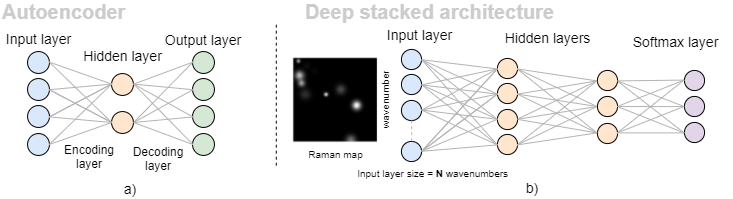
\includegraphics[width=1\textwidth]{figures_4/setup_diagram.png}
  \caption{a) shows a regular autoencoder consisting of an encoding and decoding layer. b) shows the deep stacked architecture with nonnegative constraints used for this work. Spectrum of each Raman map, consisting of 1000 wavenumbers is given as input. }\label{fig:setup}
\end{figure*}

\section{Setup}
\label{sec:setup}

As proposed in \cite{Hosseini-Asl2016} and \cite{Vincent}, a layer-wise training is used to pre-train each layer unsupervised such that features are learned. In this work, the deep nonnegative constrained autoencoder (NCAE) is replicated using the layered training approach. This means each layer of the deep architecture is trained individually, using a stacked approach. In other words, the hidden activations of the previous trained autoencoder is used as input for the next. The final autoencoder is used as input to a softmax classifier. After the individual stacked training approach, the whole network is combined and trained in a supervised fashion, e.g. finetuned. The authors propose the use of a batch gradient descent algorithm called Limited-memory BFGS (L-BFGS) quasi-Newton method which approximates the hessian matrix. However, since the implementation was done in TensorFlow (TF) a native TF optimizer, e.g. Adam, was used instead. 

\subsection{Verification}

For checking that indeed the deep-learning model, NCAE, is implemented correctly, a verification using the MNIST data set has been produced. The parameters used in the verification are the same as in \cite{Hosseini-Asl2016} with the exception of the nonnegativity constraint penalty, $\alpha$ which is changed. For illustration, the used parameters are displayed in Table \ref{tab:parameters},

\begin{table}[h]
	\centering
\begin{tabular}{l*{6}{c}r}
	\hline
	Parameters             & NCAE \\
	\hline
	Sparsity penalty ($\beta$) & 3  \\
	\hline
	Sparsity parameter (p)            & 0.05  \\
	\hline
	Weight decay penalty ($\lambda$)           & -  \\
	\hline
	Nonnegativity constraint penalty ($\alpha$)     & 0.1  \\
	\hline
	Convergence tolerance    & 1e-9  \\
	\hline
	Maximum No. of Iterations & 400 \\
	\hline
\end{tabular}
   \caption{NCAE parameters used for verification using MNIST data}
\label{tab:parameters} 
\end{table}

The latent space after finetuning is displayed in Fig. \ref{fig:separationMNIST}. As it can be observed, the handwritten digits are better separated in the second layer.
\begin{figure}[H]
	\centering
%	\includegraphics[width=1\linewidth]{figures_3/latent_space_finetune_no_legend.png}  
	\includegraphics[width=1\linewidth]{latent_space_finetune_no_legend.png}  
	\caption{MNIST latent space after finetuning}
	\label{fig:separationMNIST} 
\end{figure}

We also created a confusion matrix, Fig. \ref{fig:confusionMNIST}. The classification percentages are very high (greater and equal to 95\%) for both the validation and test datasets. This indicates that indeed the model works as hoped.

\begin{figure}[H]
%	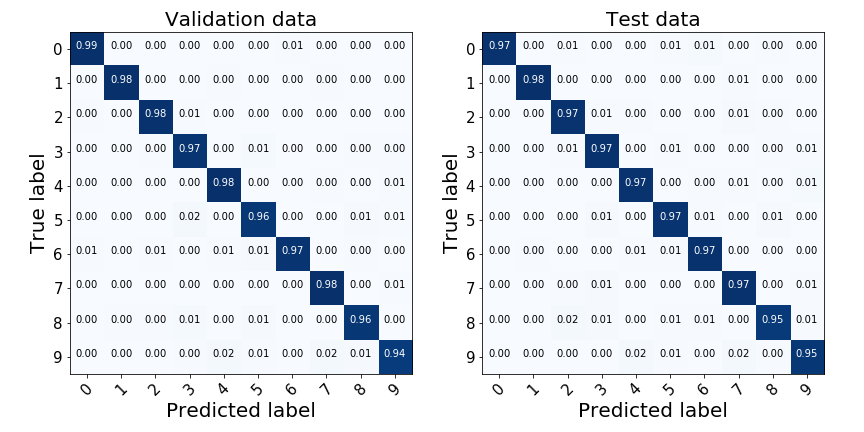
\includegraphics[width=1\linewidth]{figures_3/Confusion_matrix_fine_tune.png}  \\
   \centering
	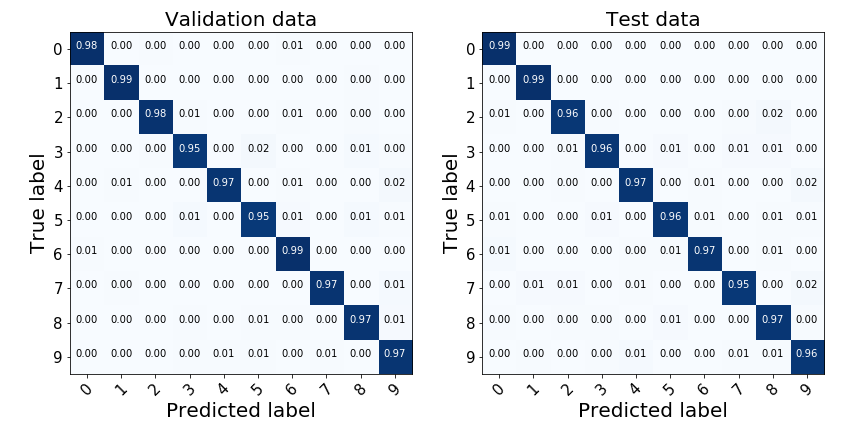
\includegraphics[width=1\linewidth]{Confusion_matrix_fine_tune_2.png}  
	\caption{MNIST confusion matrix}
	\label{fig:confusionMNIST} 
\end{figure}


\subsection{Simulated Raman data}
A simulated SERS dataset is created using MATLAB. The dataset is created using parameters such as the number of wavenumbers, and the size of the Raman map with additional parameters such as; a) Signal-to-background-ratio (SBR) that determines the intensity of the peaks with respect to the background. b) $K$ the number of Voight-profiles, e.g. the number of "substancens" or components in the spectrum and c) the number of hotspots in each Raman map.

The dataset used for training consisted of 1000 wavenumbers using a Raman map size of 100 $\times$ 100 samples. The number of hotspots was 10 with an SBR of 0 dB. Measurement noise was given as $10^{-3}$. Two different substances were created using the same parameters, however varying $K$. The resulting training data, Raman spectra, consisting of $K=1$ and $K=2$ can be observed in Fig. \ref{fig:raman} on the top most subplots. These are for the remainder of the paper referenced as Component 1 and Component 2.

The test data is a mixture of both components with an added "anomaly" to the spectrum. This is to emulate a nonlinearity in the spectra when mixing components. The mixture levels are given in steps of 10\%, e.g. one test set consists of 10\% of Component 1 with 90\% of Component 2, and so on.\\
The simulated hotspots can be visualized in Fig. \ref{fig:hotspots}.

\begin{figure}[H]
    \centering
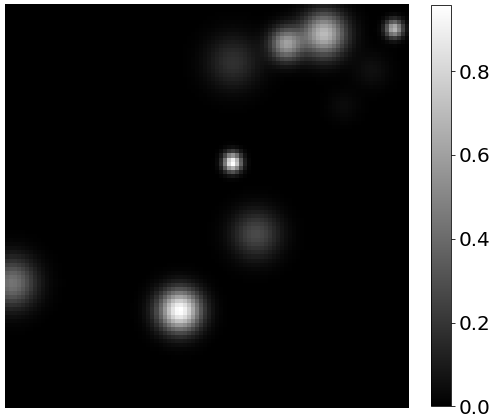
\includegraphics[width=0.5\linewidth]{figures_3/raman_sim_hotspots.png}  
\caption{Hot spots}
\label{fig:hotspots}
\end{figure}

Also, for visualization purposes, the profiles of the two "substances", class 0 and class 1, and the background signal, class 2, are displayed in Fig. \ref{fig:raman}.

\begin{figure}[H]
	\centering
%	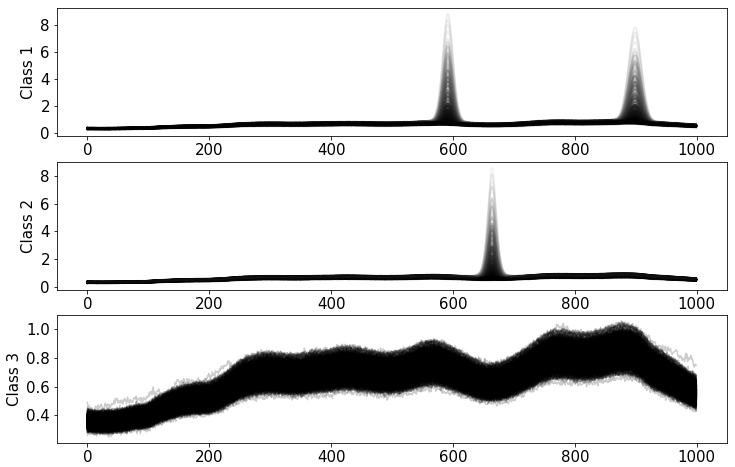
\includegraphics[width=1\linewidth]{figures_3/raman_sim_training_data_2.png}  
	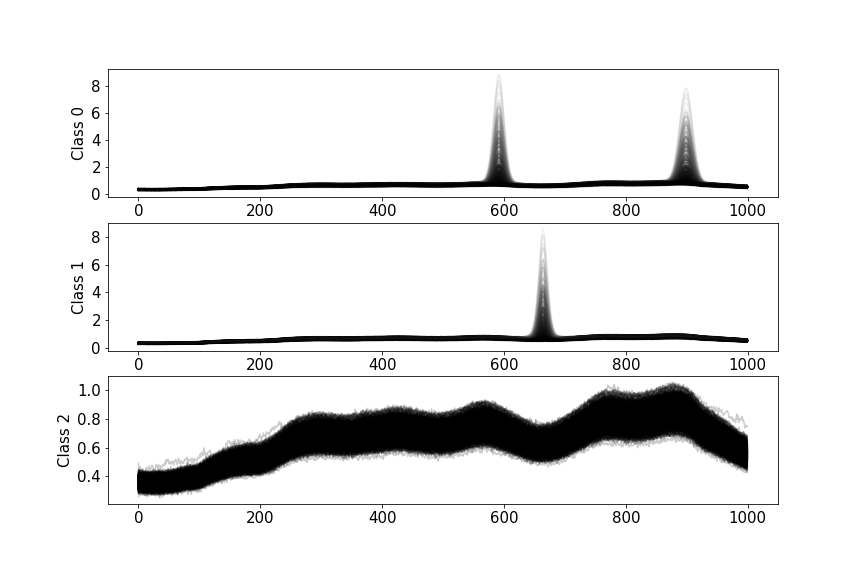
\includegraphics[width=1\linewidth]{raman_sim_training_data_2.png}  
	\caption{Raman simulation data}
	\label{fig:raman}
\end{figure}

\section{Results}
\label{sec:results}
This section contains the main results of the deep learning model described in the Setup Section \ref{sec:setup} for the simulated raman data set.\\
As described, the model is a classification model with three classes with class 2 used for collecting the background signal. \\%. One of the classes is used for collecting the background signal.\\
In order to check that indeed the model works as expected, several testing figures have been generated. These figures are presented below with a small description.\\
The first indication that the model functions correctly is the component identification. In terms of peak and wave numbers the components in Fig. \ref{fig:components} look very similar to the ones described in the Setup Section \ref{sec:setup}, Fig. \ref{fig:raman}. 
\begin{figure}[H]
	\centering
%	\includegraphics[width=0.4\textwidth]{figures_3/raman_sim_3_encode_layer_1_finetune_13.png}
	\includegraphics[width=0.4\textwidth]{raman_sim_3_encode_layer_1_finetune_13.png}
	\caption{Component identification}
	\label{fig:components}
\end{figure}
%
The weights for the second layer and softmax layer are visualized in Fig. ~\ref{fig:weights}. From Fig. \ref{fig:components} we see that units 1 and 2 are related to class 1. Further we see that these are related to components 3 and 1 + 2. Comparing Fig. \ref{fig:raman} to Fig. \ref{fig:hotspots} it is easily seen that this is class 1. The same can be done for class 0. In Figure ~\ref{fig:weights} we also see that activations go down for units 1 + 2 as the concentration of class 0 goes up and vice versa for unit 0.\\ 
% JSL: See below
%
\begin{figure}[H]
%  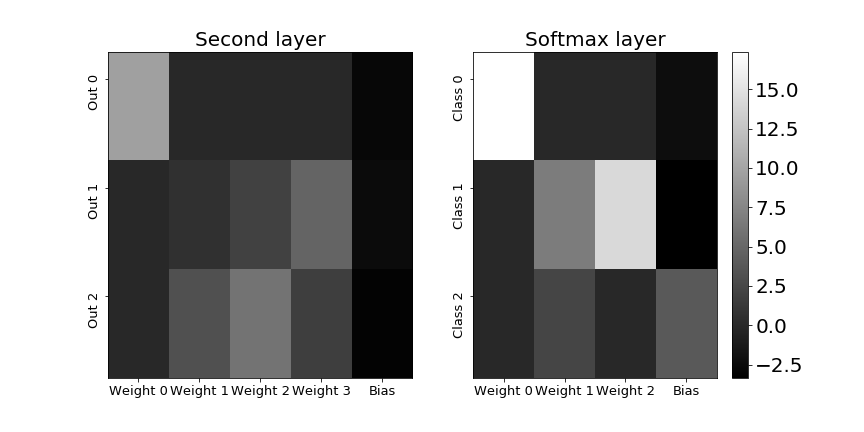
\includegraphics[width=0.5\textwidth]{figures_2/raman_sim_second_softmax_encode.png}
  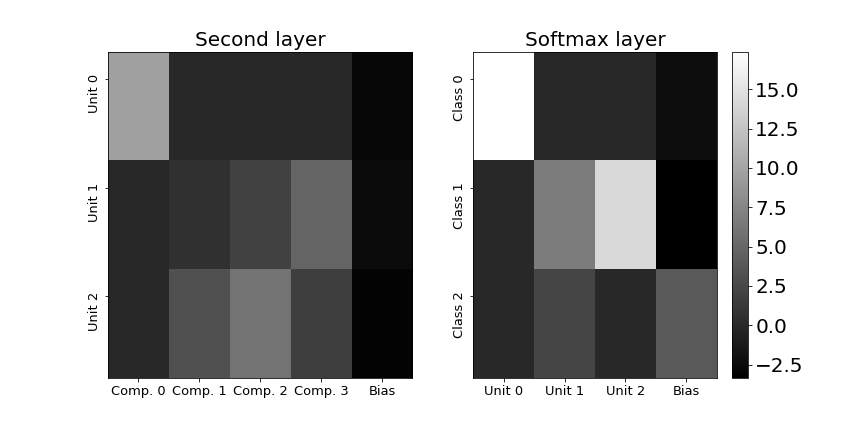
\includegraphics[width=0.5\textwidth]{raman_sim_second_softmax_encode_2.png}
  \caption{Weights for the second and softmax layers}
  \label{fig:weights}
\end{figure}
%
An overall overview of the activations and probabilities over the D space can be viewed in Fig. ~\ref{fig:activations}. As it can be observed, the hot spots are activated (lighter tones) in both images similarly to the original hot spot simulation image, Fig. ~\ref{fig:hotspots}. For probabilities, the values are slightly biased towards class 1 (even though the concentration of class 0 is 0.9, it is still concluding that class 1 is present	in the center of the hot spots). %%Class 0 and class 1 represent the two substances while class 2 represents the background. Therefore, one might say that the model performs as expected. HOW TO EXPLAIN THE SIGMOID?

%% JSL: Simple: from Figure 6 we see that units 1 and 2 are related to class 1. Further we see that these are related to comp. 3 and 1+2. Comparing Fig 5 to Fig 4 it is easily seen that this is class 1. The same can be done for class 0. In Figure 7 we see that the activations goes down for units 1+2 as the concentration of class 0 goes up and vice versa for unit 0
%% Probabilities are a bit more difficult. I think is has to do with the fact that the parameter from unit 0 to class 0 is 17.37, while the parameters from units 1 and 2 to class 1 is 6.74 and 14.22 (20.96 in total). But don't you think it is enough to state that it is slightly biased towards class 1 (even though the concentration of class 0 is 0.9, it is still concluding that class 1 is present	in the center of the hot spots)
\begin{figure}[H]
	\centering
%  \includegraphics[width=1\linewidth]{figures_3/DNN_prop_sigmoid_im.png}
%  \includegraphics[width=1\linewidth]{DNN_prop_sigmoid_im.png}
	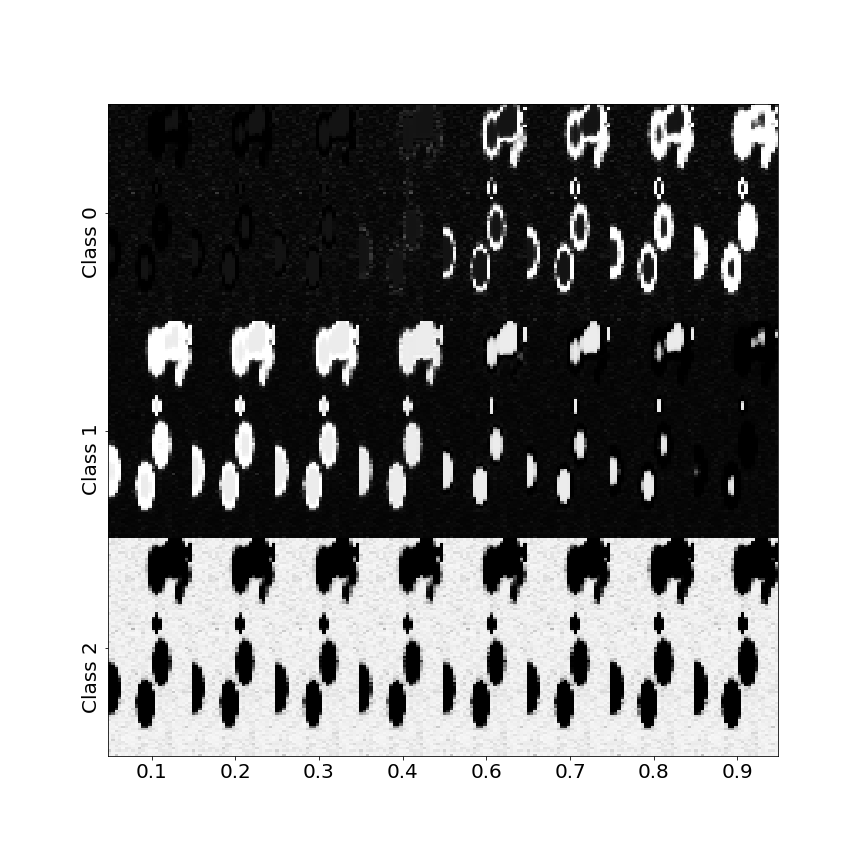
\includegraphics[width=0.25\textwidth]{DNN_prop_im.png} \hspace*{-.5cm}
	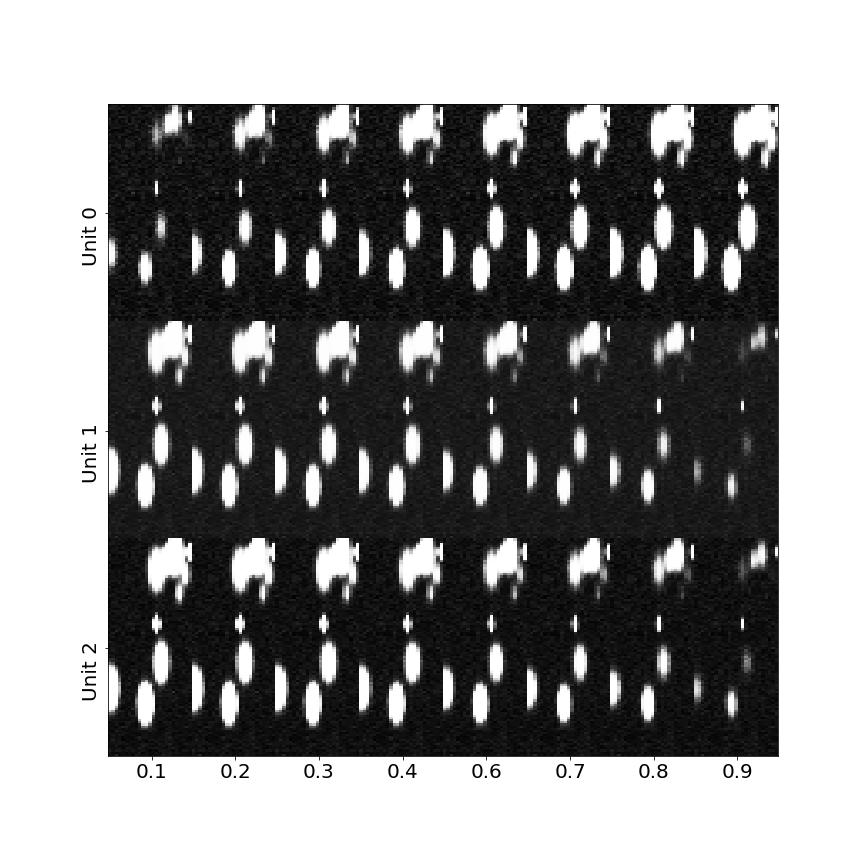
\includegraphics[width=0.25\textwidth]{DNN_sigmoid_im.png}
%  \caption{Activations}
	\caption{Left is the probabilities of each class, to the right is the activation of each hidden unit when changing the concentration of each substrate.}
    \label{fig:activations}
\end{figure}
%
We also plotted a running average to check that indeed the probabilities for class 0, 1 and 2 (blue, green and purple solid lines) over space D behave as hoped. As one can see in Fig. ~\ref{fig:Dspace}, the behaviour is consistent with Fig. ~\ref{fig:activations}.
% JSL: Perhaps not "expected", what about "hoped"?
%
\begin{figure}[H]
	\centering
%	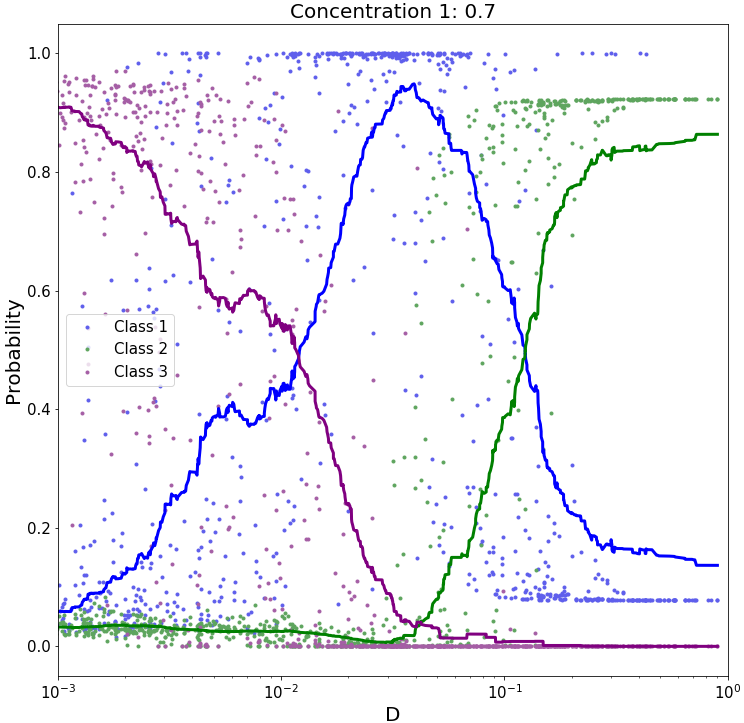
\includegraphics[width=0.3\textwidth]{figures_3/DNN_D_vs_prob_6.png}
	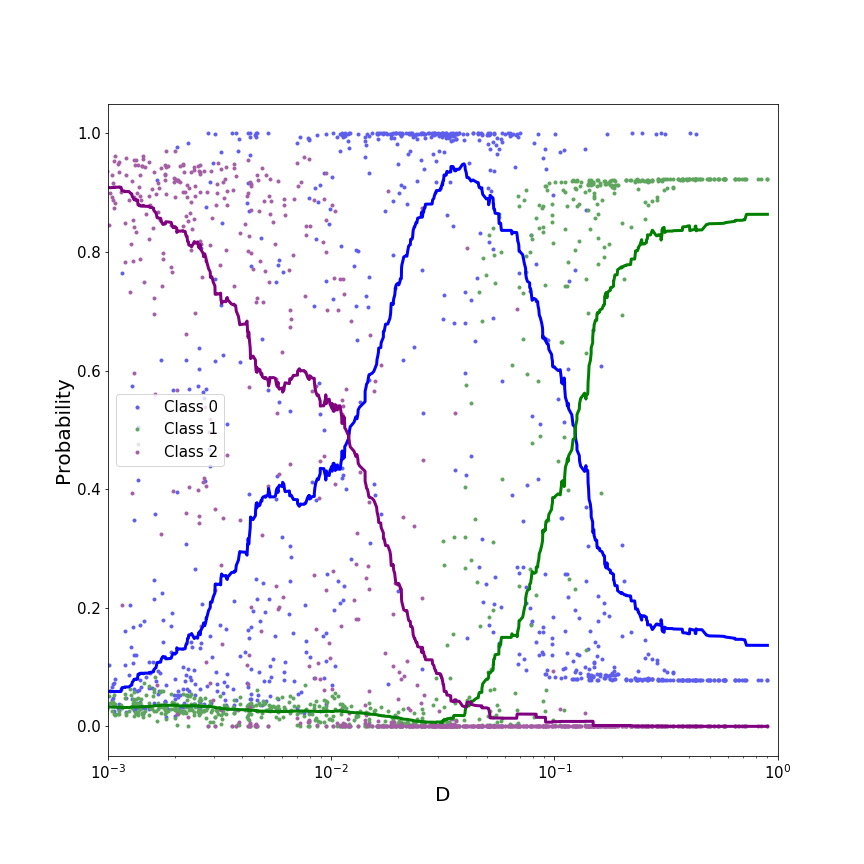
\includegraphics[width=0.25\textwidth]{DNN_D_vs_prob_6_2.png} \hspace*{-.5cm}
	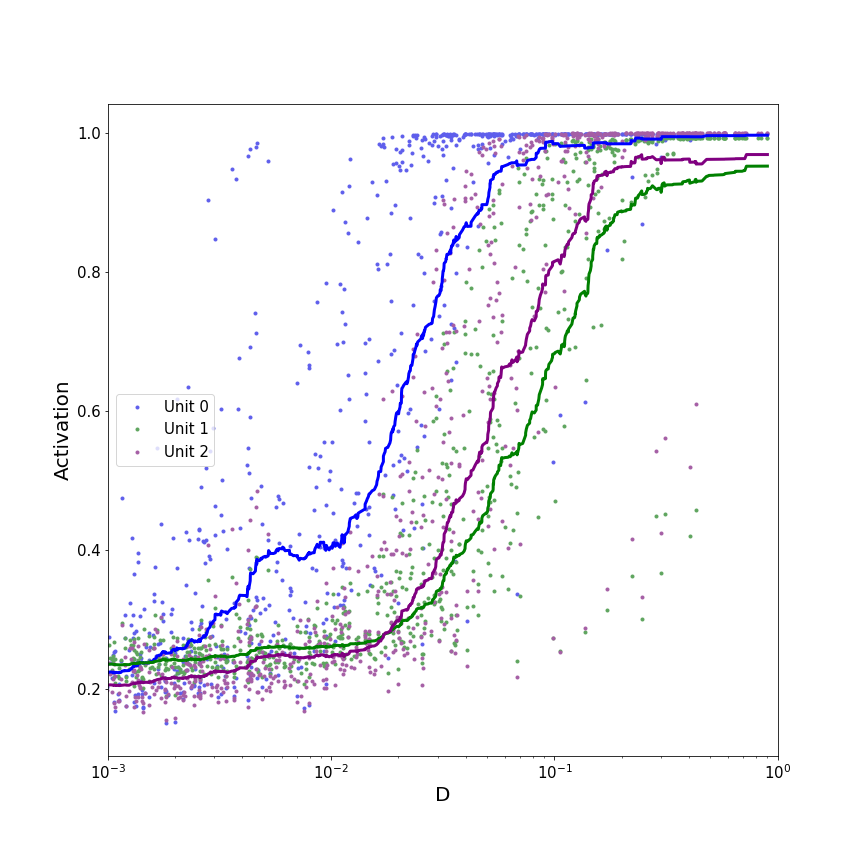
\includegraphics[width=0.25\textwidth]{DNN_D_vs_act_6.png}	
	\caption{Probability versus D space for a concentration of 0.7 for class 0 and 0.3 for class 1. Lines are running averages with a window size of 100.}
	\label{fig:Dspace}
\end{figure}
%
We plotted the confusion matrices for the test and training data, Fig. \ref{fig:confusion}. When investigating the missclassifications, we find that when $D > 6\cdot 10^{-3}$, the model is predicting correctly. This indicates another tuning parameter should be used in terms of the threshold defining the background described in the Setup Section \ref{sec:setup}.

%We also plotted the confusion matrix for classification, Figure ~\ref{fig:confusion}. The value of 0.81 for the background signal class (class 2) indicates that further tuning of parameters needs to be done. The higher the classification percentage of the background signal, the better the model will identify correctly the two substances. %PROBLEM: THE CLASS LABELS CHANGE THROUGHOUT THE FIGURES. SOMETIMES, 1,2,3 OTHERS 0,1,2 + HARD TO SEE WHICH IS WHICH. %%JSL: Fixed

%% JSL: SORRY, by mistake I reversed the input when computing the confusion matrices. 

%% Well, I'm not quite sure if that is correct. When investigating just a bit, it is clear that the model is actually predicting correct (I've traced the indicies back to the original dataset, 
\begin{figure}[H]
  \centering
%  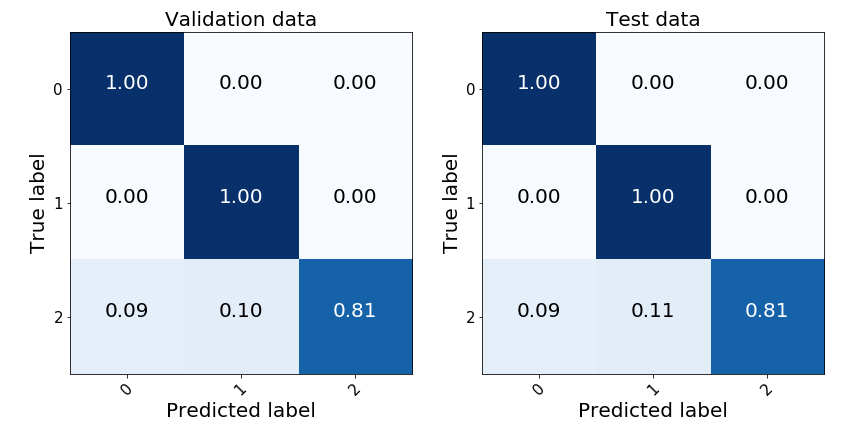
\includegraphics[width=0.5\textwidth]{figures_2/raman_sim_3_conf_matrix13.png}
  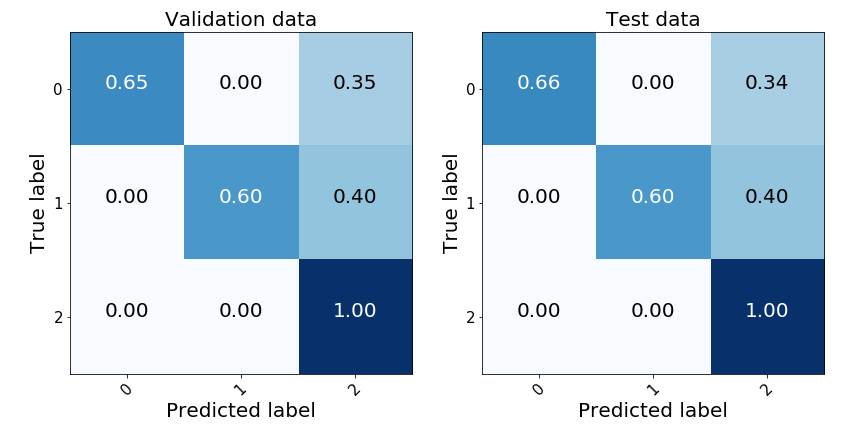
\includegraphics[width=0.5\textwidth]{raman_sim_3_conf_matrix13_2.png}
  \caption{Confuson matrix for the Raman data}
  \label{fig:confusion}
\end{figure}
%
In order to check how the model deals with the concentrations, we also made a predicted concentration using a simple transformation of the activations, Fig. ~\ref{fig:conc_sigmoids}. As the figure shows, the model performs quite poorly since the intersection should be close to the gray diagonals. %WEIRD SPACING, TRIED SOME THINGS BUT IT DOESN'T WORK.
% JSL: If you mean the spacing below Figure 10, then it is because Latex tries to fill the entire page
\begin{figure}[H]
	\centering
%	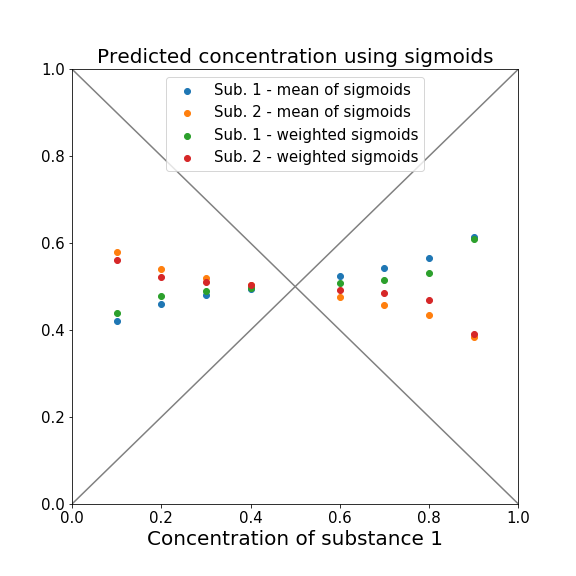
\includegraphics[width=0.26\textwidth]{figures_2/DNN_pred_conc_sigmoid.png} 
	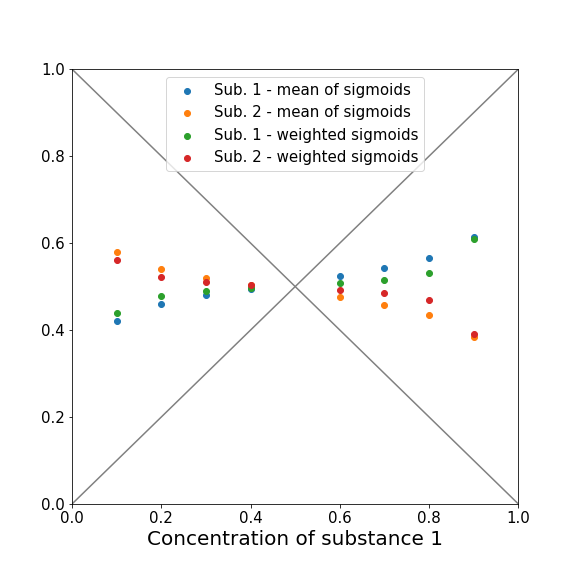
\includegraphics[width=0.26\textwidth]{DNN_pred_conc_sigmoid_2.png} 
	\caption{Predicted concentration using activations from the sigmoid function}
	\label{fig:conc_sigmoids}
\end{figure}
%
Finally, we also generated a comparison between NMF and the deep learning model for predicting concentrations, Fig. ~\ref{fig:comparison}. As it can be seen in the figures, NMF performs much better than the deep learning model. The difference between these results is described into depth in the Discussion Section ~\ref{sec:discussion}.
\begin{figure}[H]
%	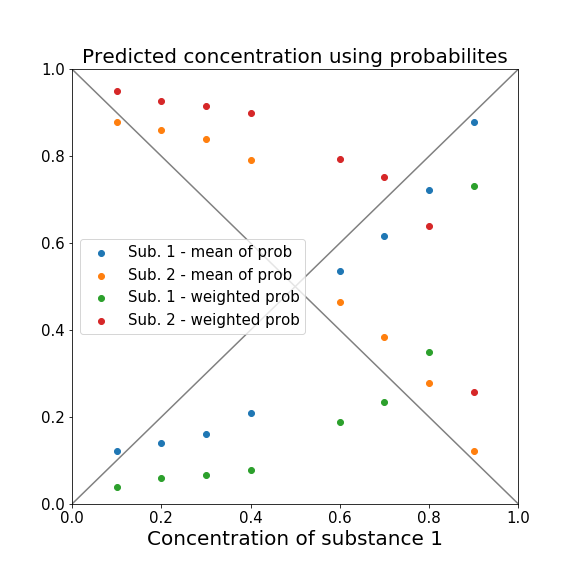
\includegraphics[width=0.23\textwidth]{figures_2/DNN_pred_conc_prob.png}
%	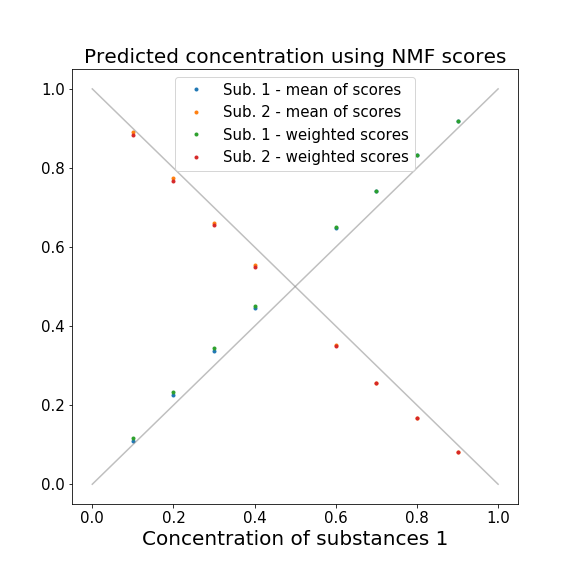
\includegraphics[width=0.23\textwidth]{figures_2/nmf_pred_conc.png}
	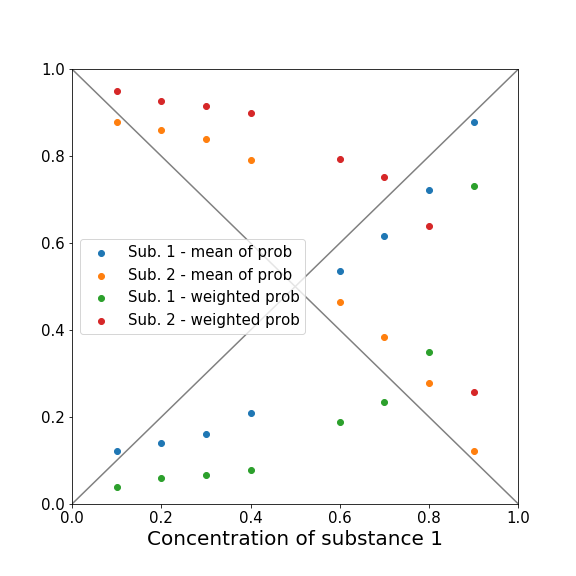
\includegraphics[width=0.25\textwidth]{DNN_pred_conc_prob_2.png} \hspace*{-.5cm}
	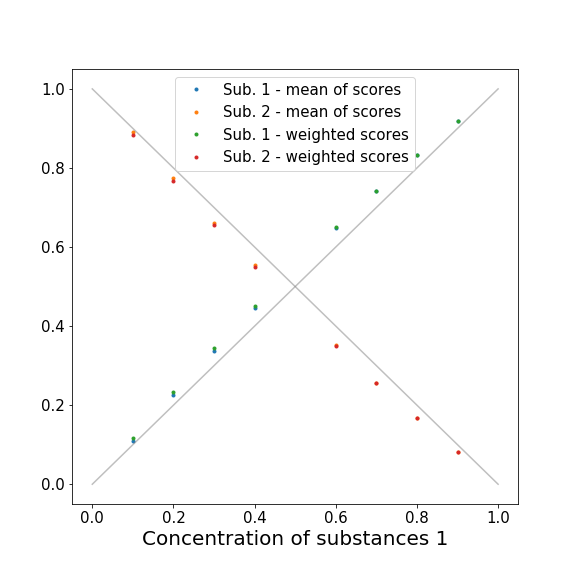
\includegraphics[width=0.25\textwidth]{nmf_pred_conc_2.png}
	\caption{Predicted concentration using probabilities (left) and NMF (right)}
	\label{fig:comparison}
\end{figure}
\section{Discussion}
\label{sec:discussion}
%JSL: Skal afsnittene rykkes om?
The estimated components shown in Fig. \ref{fig:components} are essential peak detections, which is sufficient for a classification task. It is clear that the estimated components are not strictly non-negative. This is due to the non-negative formulation \eqref{eq:non_neg} being a soft-constraint, which is in contrast to the usual hard-constraint (projection) formulation used in NMF. A way to improve this is to use the same update strategy as Seung and Lee \cite{Seung1999}. Besides achieving strict non-negativity this also has the advantage that we decrease the number of hyper parameters that has to be tuned.

Intuitively, a 3 component NMF would be able to reconstruct the the two signals in our data (one extra component is needed for the background). When using NCAE we were unable to achieve a satisfying first layer using only 3 components and needed to use 4 instead. As the background doesn't have to be modelled with the purpose of classification, this means that we end up with 3 components detecting the same peak. One solution to this would be to drop redundant components when fine tuning the final network (or even when increasing the depth of the network).

It is clear that the method to achieve a sparse solution \eqref{eq:sparse} has its drawbacks, as one way to satisfy this, is to decrease the maximum activation during training. In our experience, this is exactly what happens, at least when using a too small batch size. However, increasing the batch size too we lose the benefits of this strategy. Furthermore, when applying the method to spectroscopic data, this formulation changes interpretation when moving from pre-training to fine tuning the full network. The reason for this is, as mentioned above, the background component is no longer needed, hence a sparser solution should be searched for. An alternative to \eqref{eq:sparse} would be to apply a sparse prior to the estimated components as done in \cite{snmf2006,ramanSNMF2014}.

The resulting deep neural network is an effective classifier when detecting when there is a signal, with apparent issue illustrated in Fig. \ref{fig:confusion} being mainly an issue of tuning our threshold for creating the background class. When the network is applied to mixed data, an undesired behaviour is observed in both Fig. \ref{fig:activations} (left) and \ref{fig:comparison} (left). The probabilities for classes 0 and 1 losses their interpretation, as the Softmax function enhances even small differences in its inputs. However, in Fig. \ref{fig:activations} (right) and \ref{fig:Dspace} (right) we see that the output of the sigmoid activation functions is a non decreasing function of the amount signal (both when varying D and concentration). From Fig. \ref{fig:conc_sigmoids} and \ref{fig:comparison} (right) it is clear that a extra layer is needed in order to perform on the same level as NMF. This could be done by changing the Softmax layer into a regression layer.



\section{Conclusion}
\label{sec:conclusion}
We applied NCAE to simulated SERS data consisting of pure signals to pre-train a deep neural network with a Softmax layer on top. The resulting network was with high precision able to distinguish pure signals from each other. When we applied the network to mixed data, the output probabilities from the Softmax layer wasn't related to the actual concentrations. The sigmoid activation functions indicated that changing the last layer into a regression layer, the network would perform comparable to NMF.

% Below is an example of how to insert images. Delete the ``\vspace'' line,
% uncomment the preceding line ``\centerline...'' and replace ``imageX.ps''
% with a suitable PostScript file name.

% To start a new column (but not a new page) and help balance the last-page
% column length use \vfill\pagebreak.
% -------------------------------------------------------------------------
\vfill
\pagebreak



%\section{REFERENCES}
%\label{sec:ref}
%
%List and number all bibliographical references at the end of the paper.  The references can be numbered in alphabetic order or in order of appearance in the document.  When referring to them in the text, type the corresponding reference number in square brackets as shown at the end of this sentence .

% References should be produced using the bibtex program from suitable
% BiBTeX files (here: strings, refs, manuals). The IEEEbib.bst bibliography
% style file from IEEE produces unsorted bibliography list.
% -------------------------------------------------------------------------
\bibliographystyle{IEEEbib}
\bibliography{mendeley}

\end{document}
